\documentclass[12pt]{report}
\usepackage[T2A]{fontenc} 
%\usepackage[cp1251]{inputenc}
\usepackage[utf8]{inputenc}
\usepackage[russian, english]{babel}
\usepackage{cmap}
\usepackage{xkeyval}
\usepackage[pdftex]{graphicx}
\usepackage{amsmath}
\usepackage{amsfonts}
\usepackage{multirow}
\usepackage{xfrac}
\usepackage[labelformat=empty]{caption}
\usepackage[left=2cm,right=2cm,
     top=2cm,bottom=2cm,bindingoffset=0cm]{geometry}
     %\geometry{margin=1cm}%Just for showing, these are bad margins!
%\usepackage[pdftex]{graphics}
\graphicspath{{images/}}
\frenchspacing

%4 listing 

\usepackage{listings} %% собственно, это и есть пакет listings
\usepackage{color} %% это для отображения цвета в коде
\definecolor{mygreen}{rgb}{0,0.6,0}
\definecolor{mygray}{rgb}{0.5,0.5,0.5}
\definecolor{mymauve}{rgb}{0.58,0,0.82}
\tolerance=1000

\usepackage{caption}
\DeclareCaptionFont{white}{\color{white}} %% это сделает текст заголовка белым
%% код ниже нарисует серую рамочку вокруг заголовка кода.
\DeclareCaptionFormat{listing}{\colorbox{black}{\parbox{\textwidth}{#1#2#3}}}
\captionsetup[lstlisting]{format=listing,labelfont=white,textfont=white}

\usepackage{etoolbox}
\makeatletter
\patchcmd{\chapter}{\if@openright\cleardoublepage\else\clearpage\fi}{}{}{}
\makeatother


\begin{document}

\righthyphenmin=2
\newpage
\hfill \text{Серебро Андрей, студент  43601/2}\\

\section* {Решённые задачи}
\parindent=1cm
\newenvironment{myindentpar}[1]%
 {\begin{list}{}%
         {\setlength{\leftmargin}{#1}}%
         \item[]%
 }
 {\end{list}}
 
\subsection*{Нумерация двумерных диаграмм}
\hspace{\parindent} Повторены результаты предшественников по части нумерации двумерных диаграмм Юнга. 

Обозначим: 

\begin{itemize}
  \item $\No(\lambda)$  - номер диаграммы $\lambda$
  \item $Cells(\lambda)$  - число клеток в $\lambda$
  \item $h_\lambda(i)$ - высоту столбца с номером $i$ в диаграмме $\lambda$ (высоты считаем положительными целыми числами)
  \item $r_\lambda(i)$ - длину строки с номером $i$ в диаграмме $\lambda$
  \item $Cols(\lambda)$ - число столбцов в диаграмме $\lambda$
  \item $Y_n$ - множество двумерных диаграмм Юнга из $n$ клеток
\end{itemize}
Нумерация удовлетворяет следующим трём правилам:\\
1. Номер диаграммы из одной клетки равен 1;\\
2. Если $Cells(\lambda_1) < Cells(\lambda_2)$, то $\No(\lambda_1) < \No(\lambda_2)$;\\
3. Иначе если $Cells(\lambda_1) = Cells(\lambda_2)$ и $\exists k \ge 1 : \forall i \in \{1..k-1\} h_{\lambda_1}(i) = h_{\lambda_2}(i)$ и $h_{\lambda_1}(k) < h_{\lambda_2}(k)$, то $\No(\lambda_1) < \No(\lambda_2)$

Для того, чтобы найти номер диаграммы по этим правилам, предварительно подсчитывается $P(n, k)$ $\forall n, k \in \mathbb{N} : 0 < n < N, k < n$ - число разбиений числа $n$ на натуральные слагаемые с максимальным слагаемым, не превосходящим $k$. На данный момент число $N = 600$, так как нумерация диаграмм с большим числом клеток не требуется. Далее, для нахождения номера диаграммы, применяется Алгоритм 1.
\vspace{1cm}

Алгоритм 1 (получения номера диаграммы).

ВХОД: диаграмма $\lambda$, заданная высотами столбцов.

ВЫХОД: $\No(\lambda)$.

1. $num := 1, c := 1$ 

2. WHILE $c < Cells(\lambda)$ DO 

\hspace{1cm} $num := num + P(c, c)$

\hspace{1cm} $c := c + 1$

\hspace{0.35cm} END WHILE

3. FOR i FROM 1 TO $Cols(\lambda)$ DO

\hspace{1cm} IF $h_\lambda(i) = 1$

\hspace{2cm} BREAK

\hspace{1cm} $num := num + P(c, h_\lambda(i) - 1)$

\hspace{1cm} $c := c - h_\lambda(i)$

\hspace{0.35cm} END FOR

4. RETURN num

Оценим сложность данного метода. Пусть требуется найти номер диаграммы из $n$ клеток. $P(n, n)$ растёт как $O(\frac{exp(\sqrt(n))}{n})$, поэтому длина номера $num$ в ходе цикла WHILE растёт как $O(\sqrt{c})$, поэтому сложность этого цикла не превосходит $O(n\sqrt{n})$. Цикл FOR также требует $O(n\sqrt{n})$ времени, поэтому весь алгоритм в худшем случае исполняется за $O(n\sqrt{n}$.

\subsection*{Точный подсчёт вероятностей диаграмм}

\hspace{\parindent} Для нескольких марковских процессов на графе Юнга реализован точный подсчёт вероятностей получения диаграмм с заданным числом клеток. Сейчас присутствуют процесс Ричардсона, Планшереля, псевдопланшерелевский процесс (переходная вероятность пропорциональная $(x^2+y^2)^{0.16}$), а также псевдоричардсонский процесс (переходная вероятность пропорциональна числу исходящих дуг из вершины, переходную вероятность в которую мы считаем). 

Точные вероятности для процесса Ричардсона удается быстро посчитать для диаграмм из 70-80 клеток. Для псевдопланшерелевского процесса за короткое время для диаграмм из 70 клеток. Предельная форма псевдоричардсоновского процесса совпадают с ричардсоновским (проверено в серии экспериментов, в которых строились случайные диаграммы из 100 000 клеток).

\subsection*{Предельные формы диаграмм}

\hspace{\parindent} Для описанных выше процессов построены предельные формы (брались диаграммы из 1000 000 клеток). 

\begin{figure}[!ht]
\begin{center}
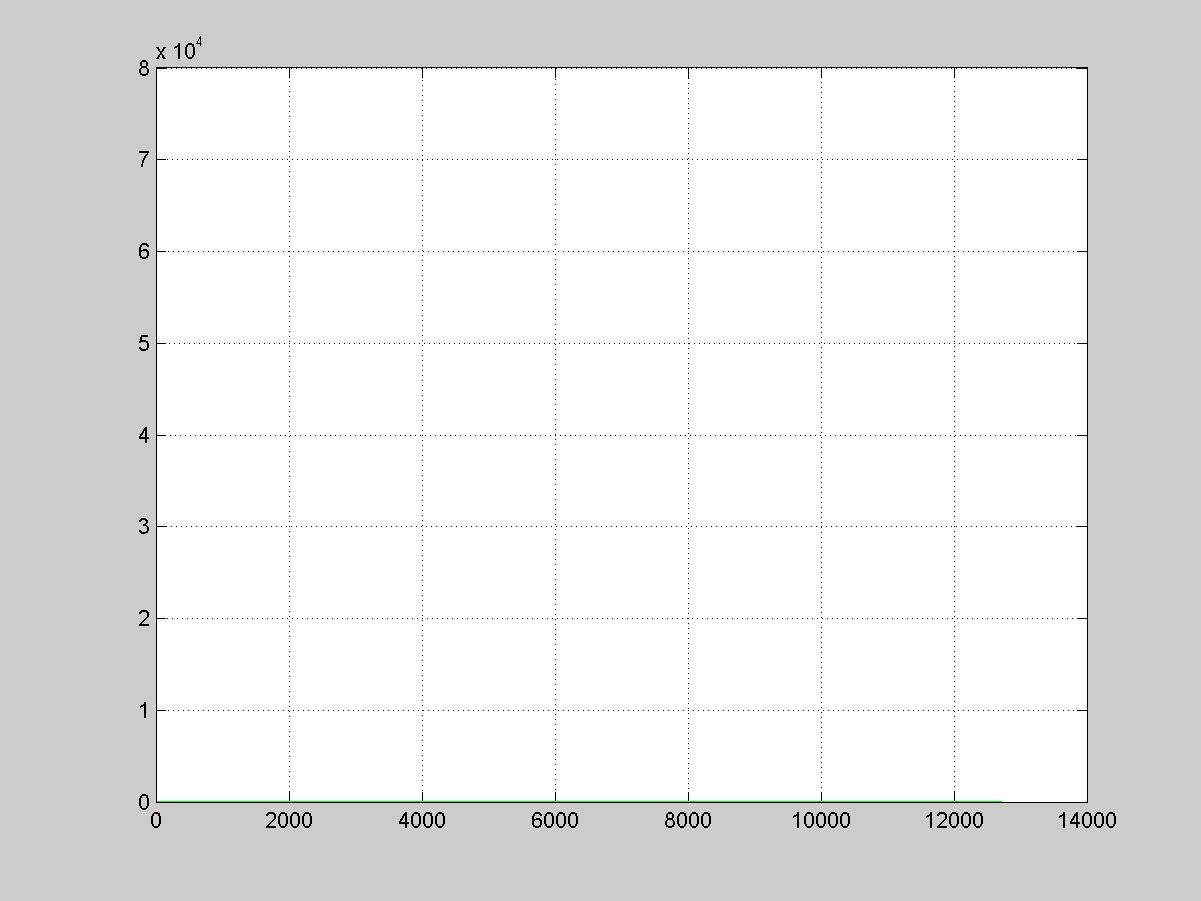
\includegraphics[scale=0.2]{Plansherel_assympt}
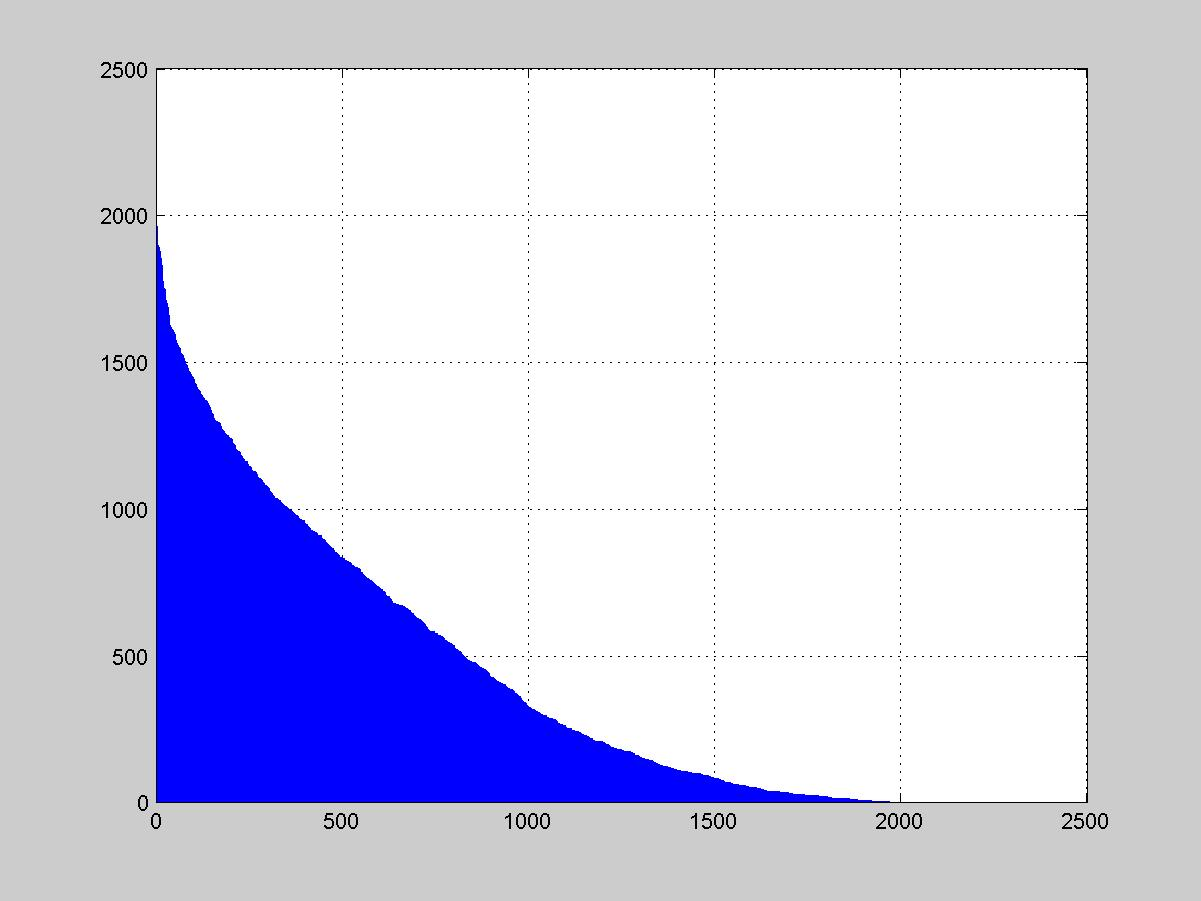
\includegraphics[scale=0.2]{ALPHA_assympt}
\\Рис. 2. Асимптотическая форма случайной диаграммы при процессе Планшереля (слева) и псевдоплашереля (справа).
\end{center}
\end{figure}

\begin{figure}[!ht]
\begin{center}
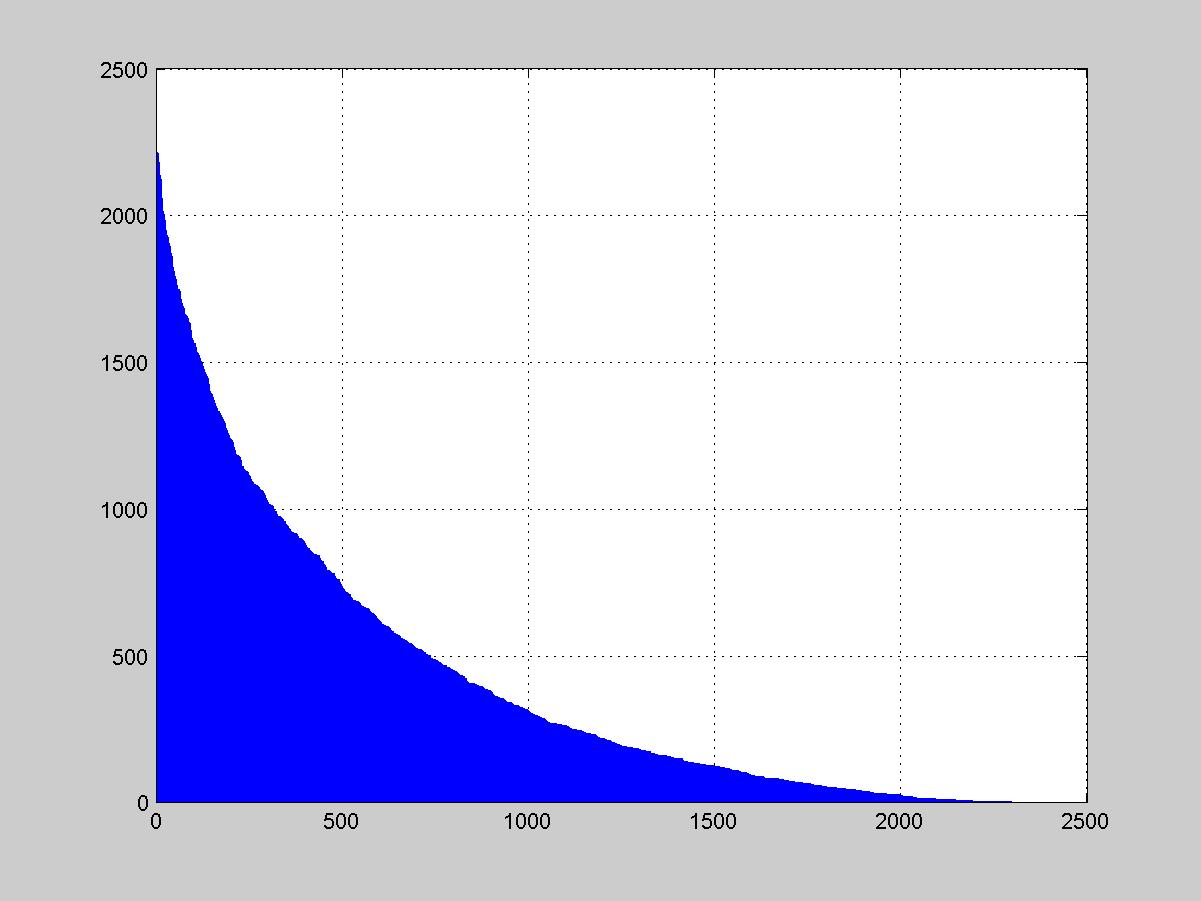
\includegraphics[scale=0.2]{Richardson_assympt}
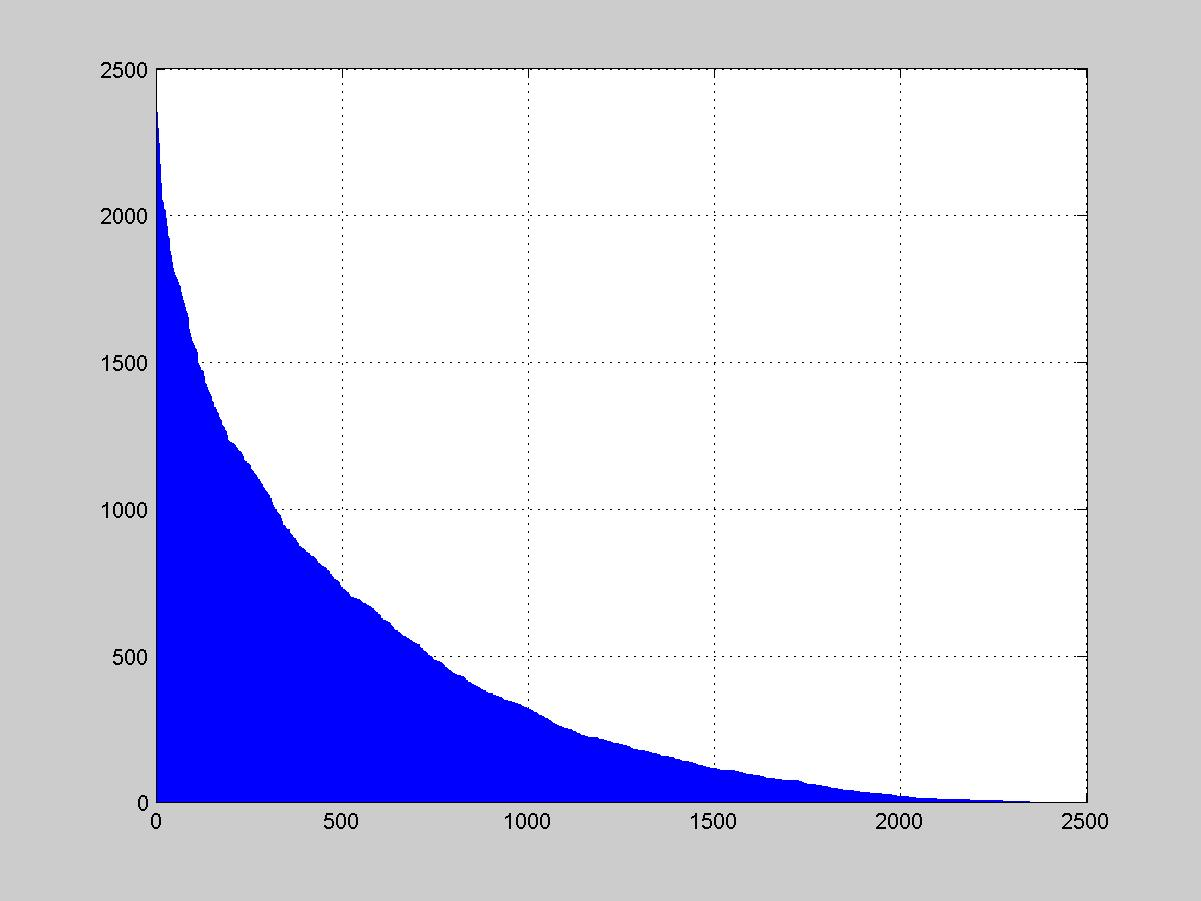
\includegraphics[scale=0.2]{Beta_assympt}
\\Рис. 3. Асимптотическая форма случайной диаграммы при процессе Ричардсона и псевдоричардсона.
\end{center}
\end{figure}

\newpage
\subsection*{Подсчёт расстояния Канторовича между диаграммами}

\hspace{\parindent} Основываясь на статье А. М. Вершика, реализован подсчёт расстояний Канторовича между диаграммами в графе Юнга. В качестве центральной меры на пространстве путей взята мера Планшереля. Проведены эксперименты (в том числе, я выяснил, что за разумное время - около получаса - можно найти расстояние между диаграммами из 50 клеток, при этом пришлось решить 36 695 768 транспортных задач.) Между диаграммами из 40 клеток расстояние ищется за время порядка 30 секунд. Также вычислены все расстояния между диаграммами на 10 этаже графа Юнга, гистограмму расстояний можно увидеть на рис. 4.

\vspace{1cm}

Алгоритм 2 (нахождения расстояния Канторовича между двумя вершинами с одного уровня градуированного графа).

ВХОД: две вершины $d_1, d_2$ одного уровня градуированного графа $G$.

ВЫХОД: $dist(d_1, d_2)$ - расстояние Канторовича между ними.

1. Создаём ассоциированный массив $distances[u, v]$, который будет содержать найденные расстояния между вершинами. Задаём расстояния на первом неединичном этаже графа и записываем их в этот массив (на первом этаже, содержащем больше одной вершины). Обозначим номер этого этажа через $s$.

2. Строим массивы вершин $V_i$ - предшественниц для $d_1$ и  $d_2$ с этажа $s \le i \le Cells(d_1)$ - для общности кода считаем вершины сами себе прдешественниками тоже. Попутно помечаем в каждой вершине поле $V.anc$, указывающее, какой вершине - $d_1$ или $d_2$ - она приходится предком. Если она приходится предком для обеих вершин, также отмечаем это (для этого с каждой вершиной достаточно ассоциировать два бита). 

3. FOR $i$ FROM $s + 1$ TO $Cols(d_1)$ DO

\hspace{1cm} FOR $v \in V_i$ DO

\hspace{2cm} $c_1 := \emptyset$

\hspace{2cm} $pred_1 := \emptyset$

\hspace{2cm} countCoefficientsForKantorovichMetric($v, c_1, pred_1$)

\hspace{2cm} FOR $u \in V_i$ DO

\hspace{3cm} IF $u.anc$ = $v.anc$ AND $u.anc$ XOR 3 = TRUE 

\hspace{4cm} CONTINUE

\hspace{3cm} $c_2 := \emptyset$

\hspace{3cm} $pred_2 := \emptyset$

\hspace{3cm} $costs := \emptyset$

\hspace{3cm} countCoefficientsForKantorovichMetric($u, c_2, pred_2$)

\hspace{3cm} FOR $p \in pred_1$ DO

\hspace{4cm} FOR $q \in pred_2$ DO

\hspace{5cm} $costs[p, q] := distances[p, q]$ 

\hspace{3cm} $x := $ solveTransportationPotential($costs, c_1, c_2$)

\hspace{3cm} $distances[u, v] := 0$

\hspace{3cm} FOR $p \in pred_1$ DO

\hspace{4cm} FOR $q \in pred_2$ DO

\hspace{5cm} $distances[u, v] := distances[u, v] + costs[p, q] \cdot x[p, q]$ 

\hspace{1cm} END FOR

\hspace{0.35cm} END FOR

4. RETURN $distances[d_1, d_2]$

\vspace{1cm}

Здесь используется функция countCoefficientsForKantorovichMetric($u, c, pred$), принимающая на вход вершину графа $u$ и возвращающая в массиве $c$ копереходные вероятности для рёбер, соединяющих $u$ c её предшественниками, а в $pred$ соответствующих предшественников $u$. Функция solveTransportationPotential решает транспортную задачу методом потенциалов. Алгоритм оптимален в том смысле, что не вычисляет расстояния, которые не требуются для определения итогового расстояния.

Сложность данного алгоритма ещё предстоит оценить. Пока что очевидно, что число решаемых транспортных задач (скорее всего) в случае графа Юнга зависит от числа клеток во входных диаграммах экспоненциально. То есть, вряд ли граф Юнга достаточно локален, чтобы число предшественников не росло быстро. 

\begin{figure}[!ht]
\begin{center}
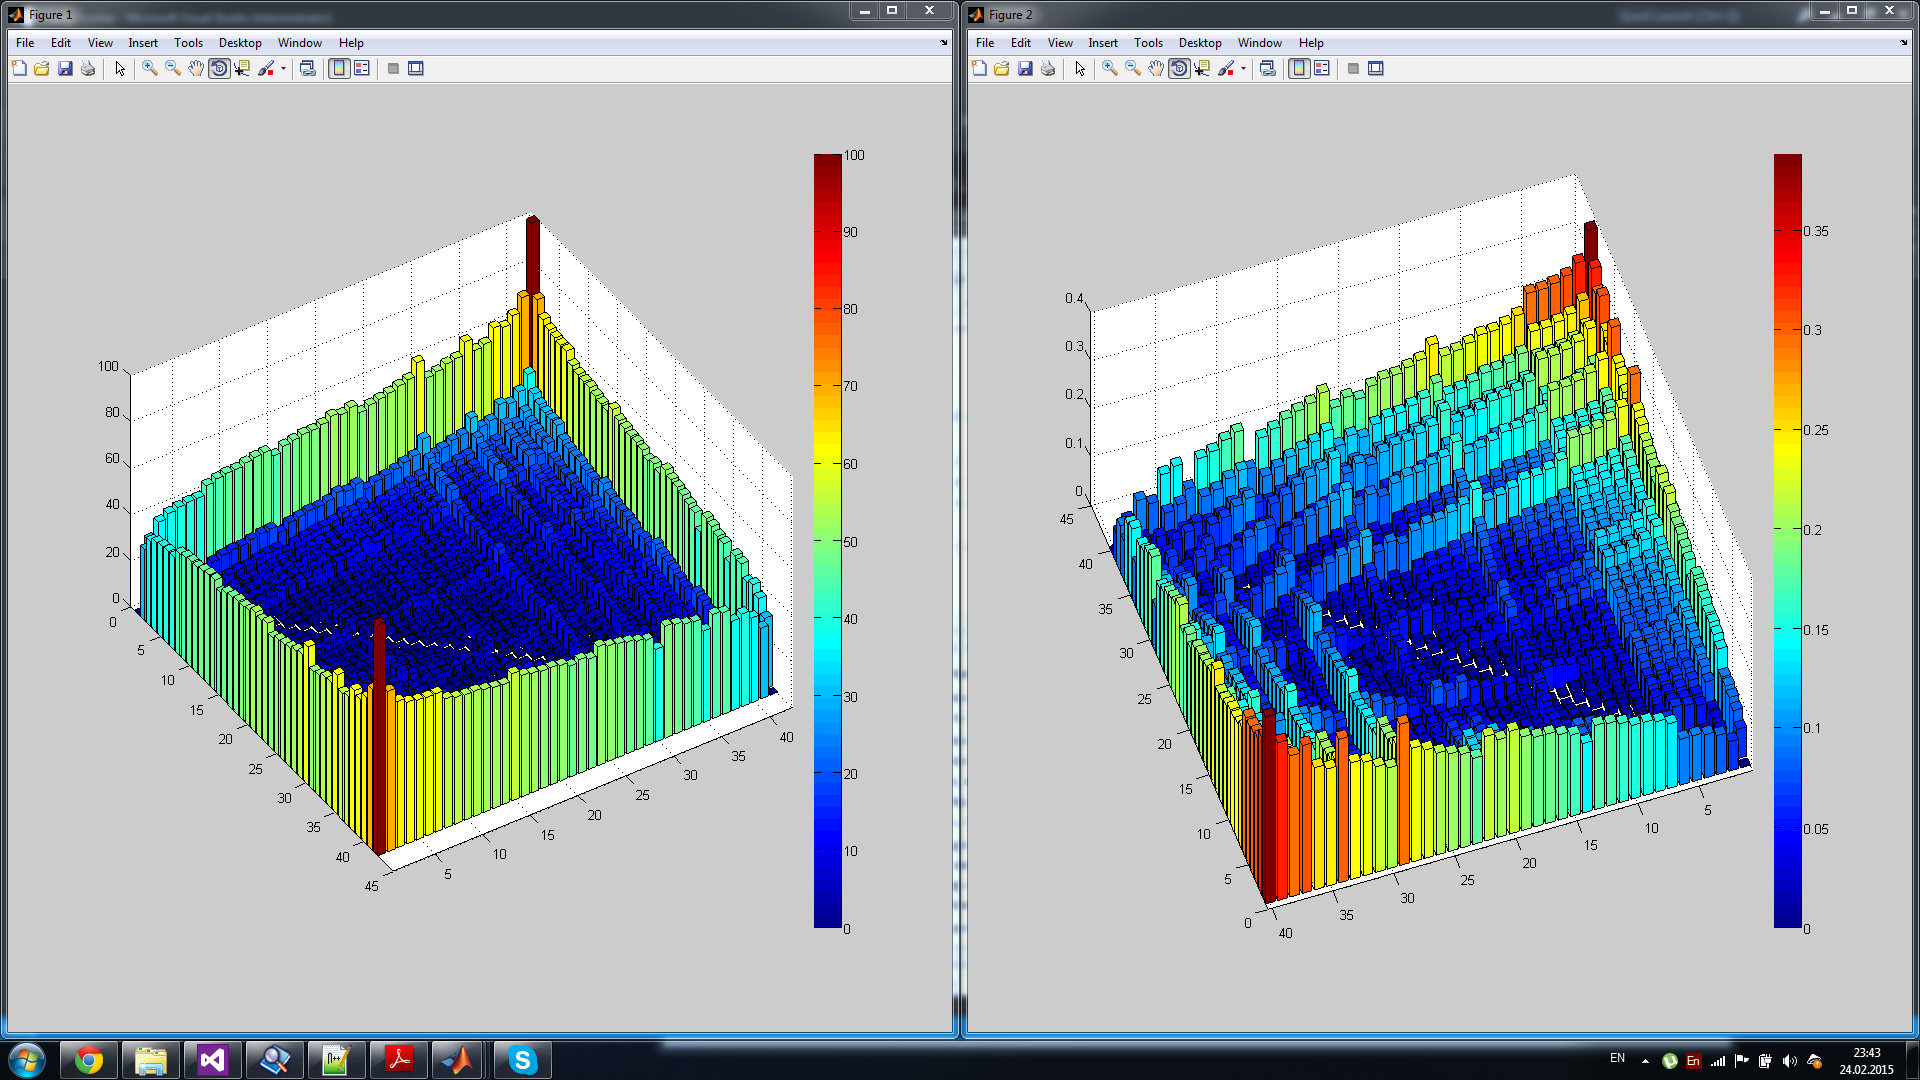
\includegraphics[scale=0.3]{metric}
\\Рис. 4. Гистограмма расстояний Канторовича между диаграммами 10го этажа графа Юнга. Правая картинка отражает расстояния между всеми диаграммами, кроме крайних, ибо они являются резкими выбросами и сглаживают картину для остальных.
\end{center}
\end{figure}

\subsection*{Метрика Канторовича на симплексе}

\hspace{\parindent} Для понимания того, как устроена метрика Канторовича, было рассмотрено расширение метрики с вершин симплекса на симплекс. Размерность симплекса выбрана два для наглядности. В результате стало понятно, что в двумерном случае шарами являются шестиугольники. Для этого я выбирал произвольную точку внутри треугольника (например, центр масс) и считал расстояния между ним и узлами сетки, на который предварительно разбил треугольник. Интересен простейший случай, когда треугольник равносторонний, то есть расстояния между всеми вершинами заданы одинаковыми. В этом случае шестиугольники точек, равноудаленных от центра масс треугольника получаются равносторонними со сторонами, параллельными сторонам треугольника (см. рис. 5). Это позволяет также выдвинуть некоторые гипотезы касательно того, как может выглядеть сфера в более высоких размерностях. Немного порисовав, я представил себе, как выглядит шар в трёхмерном случае, когда симплекс - правильный тетраэдр. Это будет четырнадцатигранник, составленный из 8 тетраэдров и 6 четырёхугольных пирамид. Картинку его я смог найти например тут: http://borgece.livejournal.com/1854.html, по запросу четырнадцатигранник. Две нижние картинки показывают метрику на равностороннем треугольнике.
Сейчас хочу попробовать экстраполировать представление шара на произвольную размерность (думаю, будет полезно для понимания структуры  шаров на графе Юнга).

Отталкиваться можно от числа гиперграней шара: число граней в зависимости от размерности выглядит так:

\begin{center}
\begin{tabular}{|c|c|c|c|c|}
\hline
Размерность симплекса & 1 & 2 & 3 & ...\\
\hline
число граней шара & 2 & 6 & 14 & ? \\
\hline
\end{tabular}
\end{center}

Быть может, в пространстве размерности $n$ число граней есть $2 (2^n - 1)$. 

С другой стороны, можно понять и, я полагаю, доказать, что при сечении шара размерности $n$ гиперплоскостями, параллельными сторонам симплекса, будет получаться шар размерности $n - 1$. Когда же сечение дойдёт до границы симплекса, оно даст в пересечении с этой границей просто симплекс размерности $n-1$. Это ещё один способ представить себе шары больших размерностей.
\begin{figure}[!ht]
\begin{center}
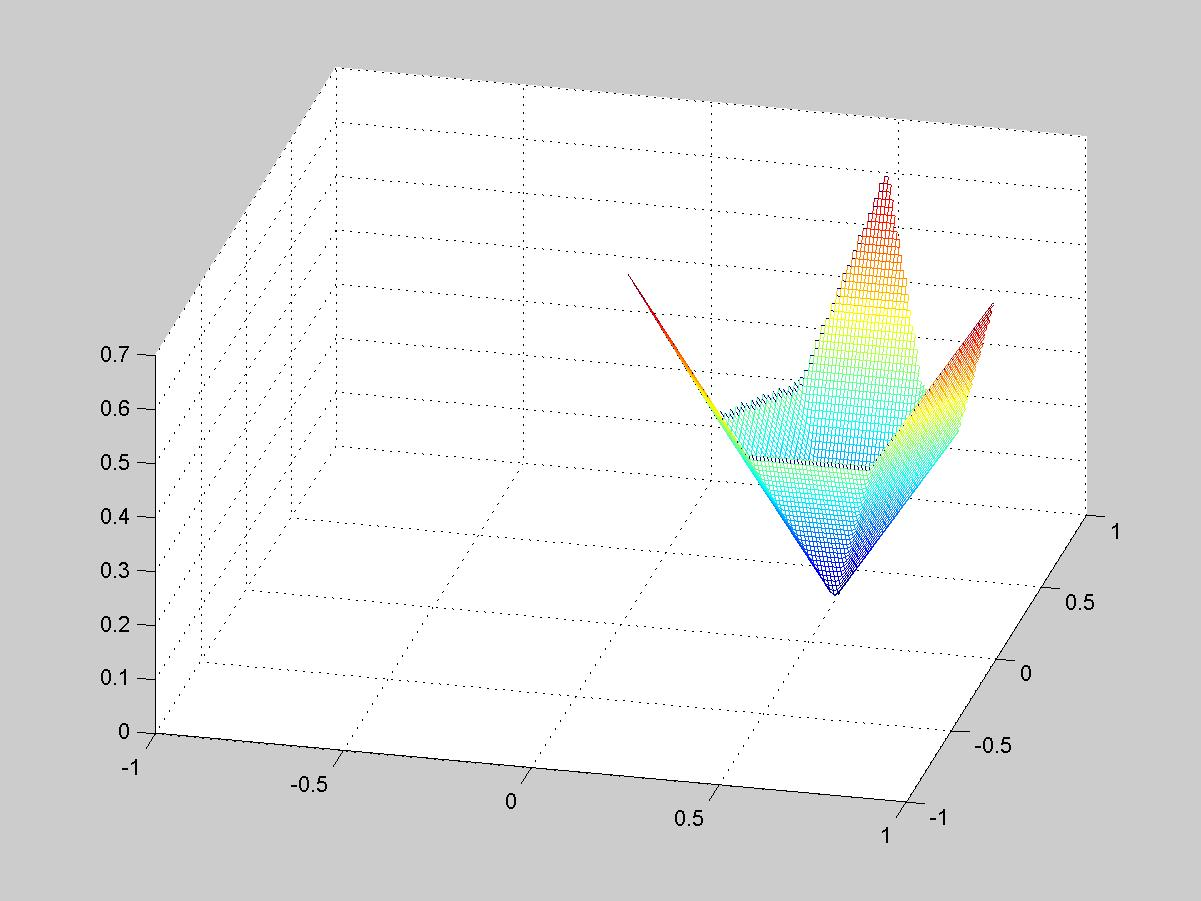
\includegraphics[scale=0.2]{SimplexDists1}
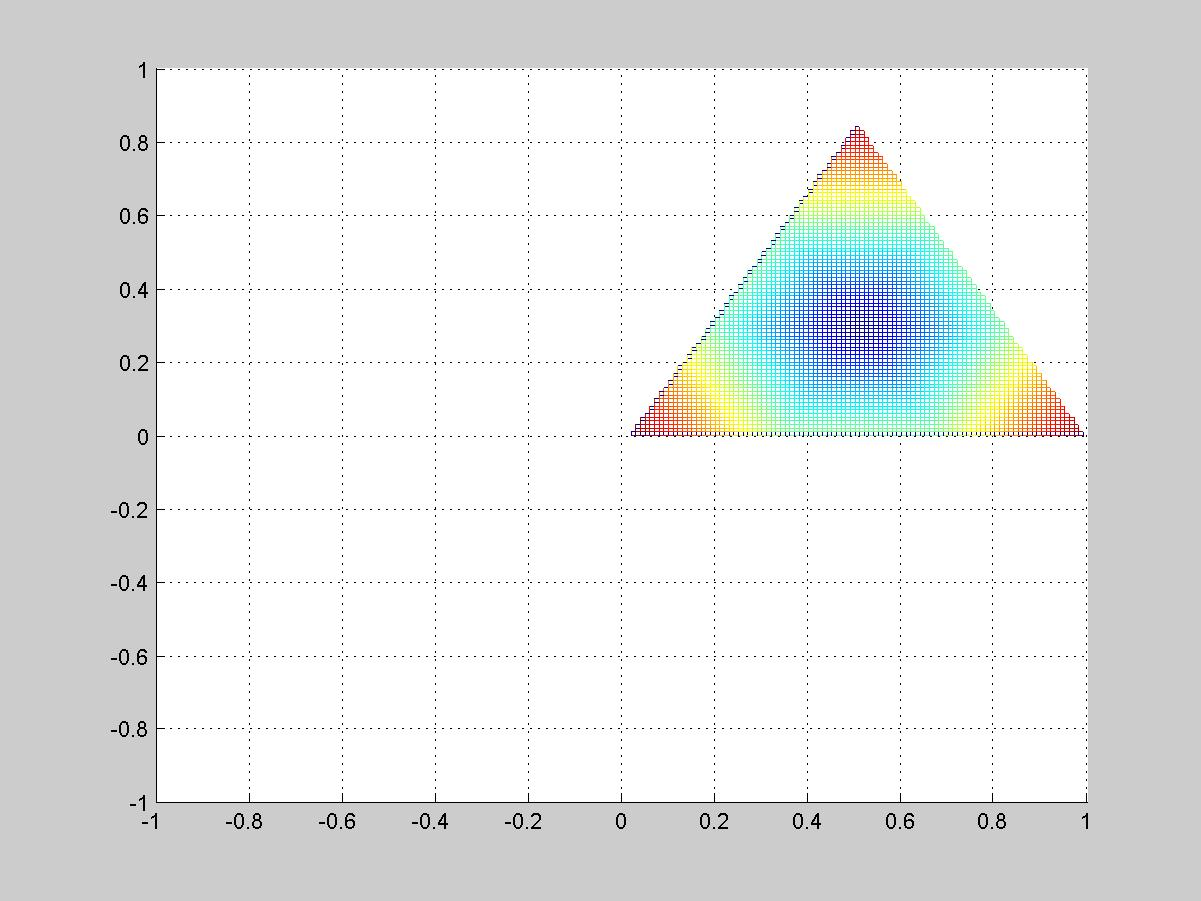
\includegraphics[scale=0.2]{SimplexDists2}
\\Рис. 5. Расстояния между центром масс равностороннего треугольника и точками треугольника. Равноудаленные точки дают одинаковый цвет графика.
\end{center}
\end{figure}


\begin{figure}[!ht]
\begin{center}
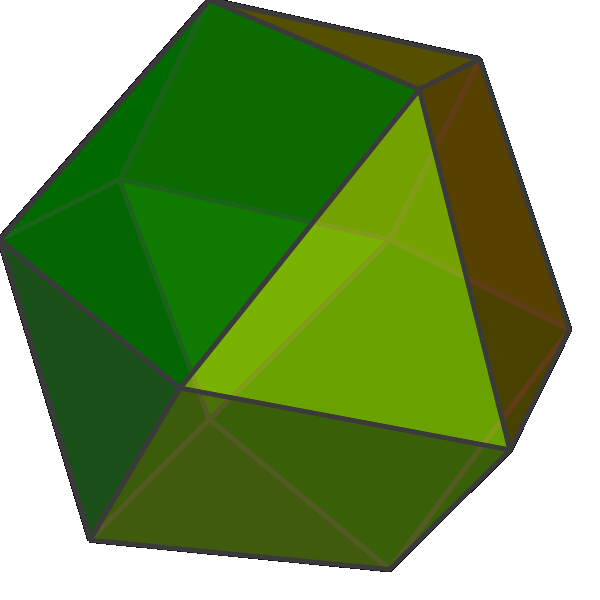
\includegraphics[scale=0.4]{14surf}
\\Рис. 6. Четырнадцатигранник (кубооктаэдр), который является шаром в трёхмерном случае. В случае правильного симплекса все его грани параллельны граням исходного симплекса (тетраэдра).
\end{center}
\end{figure}

\newpage
\subsection*{Приближение метрики Канторовича}
\hspace{\parindent} Рассмотрена гипотеза А. М. Вершика о том, что расстояние Канторовича между диаграммами $dist(\lambda_1, \lambda_2) = \sum\limits_{i = 1}^n c_i\Delta_i$, где $\Delta_i = r_{\lambda_1}(i) - r_{\lambda_2}(i)$, $c_i$ - какие-то коэффициенты, предположительно быстро убывающие с ростом $i$. Предлагается, насколько я понял, попробовать подобрать их, а также убедиться, что коэффициенты действительно быстро убывают:  например, это можно увидеть, рассмотрев расстояние между прямоугольной диаграммой и треугольной, которое видимо будет маленьким, несмотря на их непохожесть, так как первые строки у них будут иметь почти одинаковый размер. 

Сейчас решается несколько более простая задача: оценка расстояния от данной диаграммы до всех других. Приближение ищется методом наименьших квадратов путем минимизации функции невязки. Пусть взята диаграмма $\lambda$, $n = Cells(\lambda)$ и мы хотим оценить расстояние от неё до произвольной диаграммы с её уровня. Для этого решаем задачу: $c = \arg \min\limits_{c \in \mathbb{R}^n}(\sum\limits_{\lambda_i \in Y_n}(\sum\limits_{j = 1}^n c_j\Delta_{ij} - dist(\lambda, \lambda_i))^2)$, где $\Delta_{ij} = r_{\lambda}(i) - r_{\lambda_{j}}(i), i = 1..n, j = 1..|Y_n|$.

С результатами можно ознакомиться на рисунке 7 (бралась случайная диаграмма из 20 клеток и считалось расстояние от неё до всех остальных). Видно, что хотя невязка присутствует, имеется явная корреляция между $\Delta_i$ и расстоянием, что позволяет сделать вывод о возможности лучшей оценки с помощью каких-то более сложных функций от $\Delta_i$.

\begin{figure}[!ht]
\begin{center}
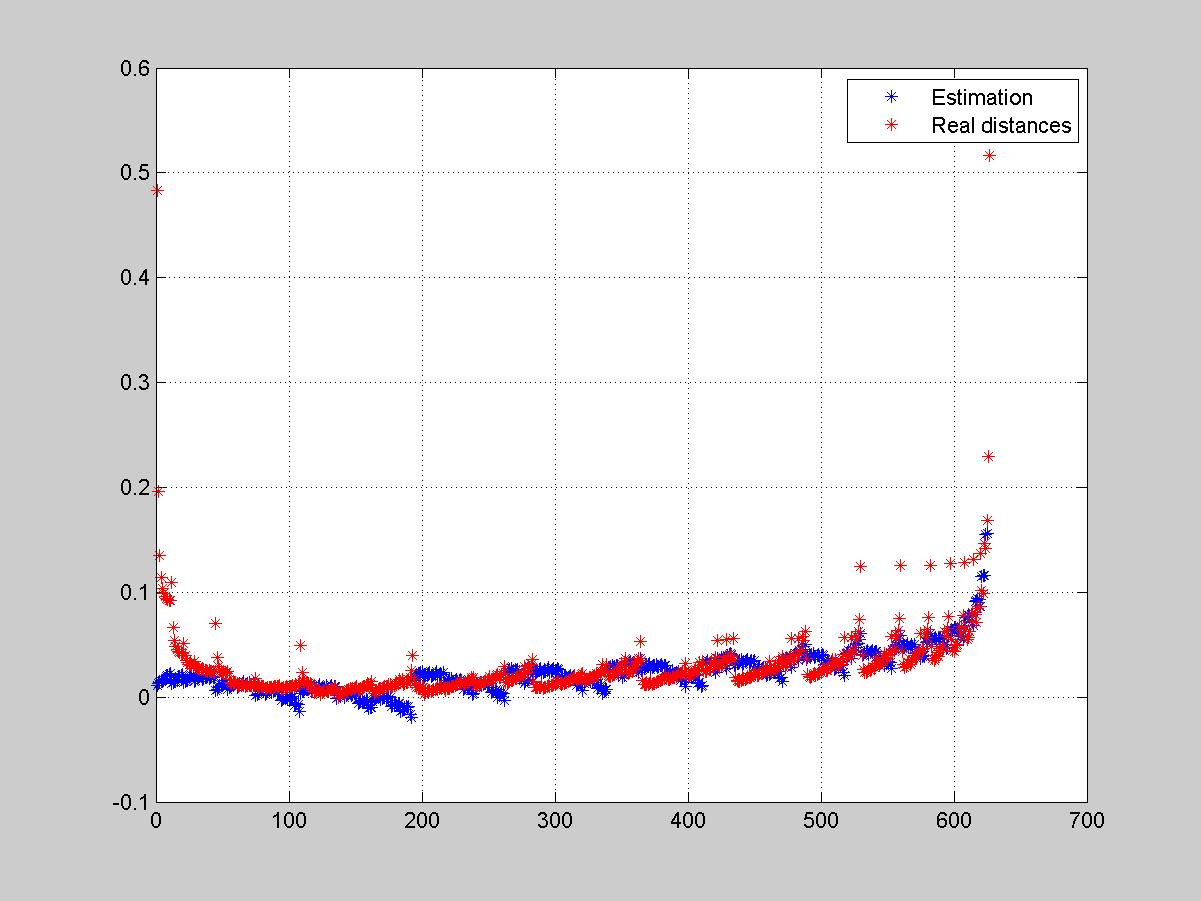
\includegraphics[scale=0.2]{MetricEstimation20}
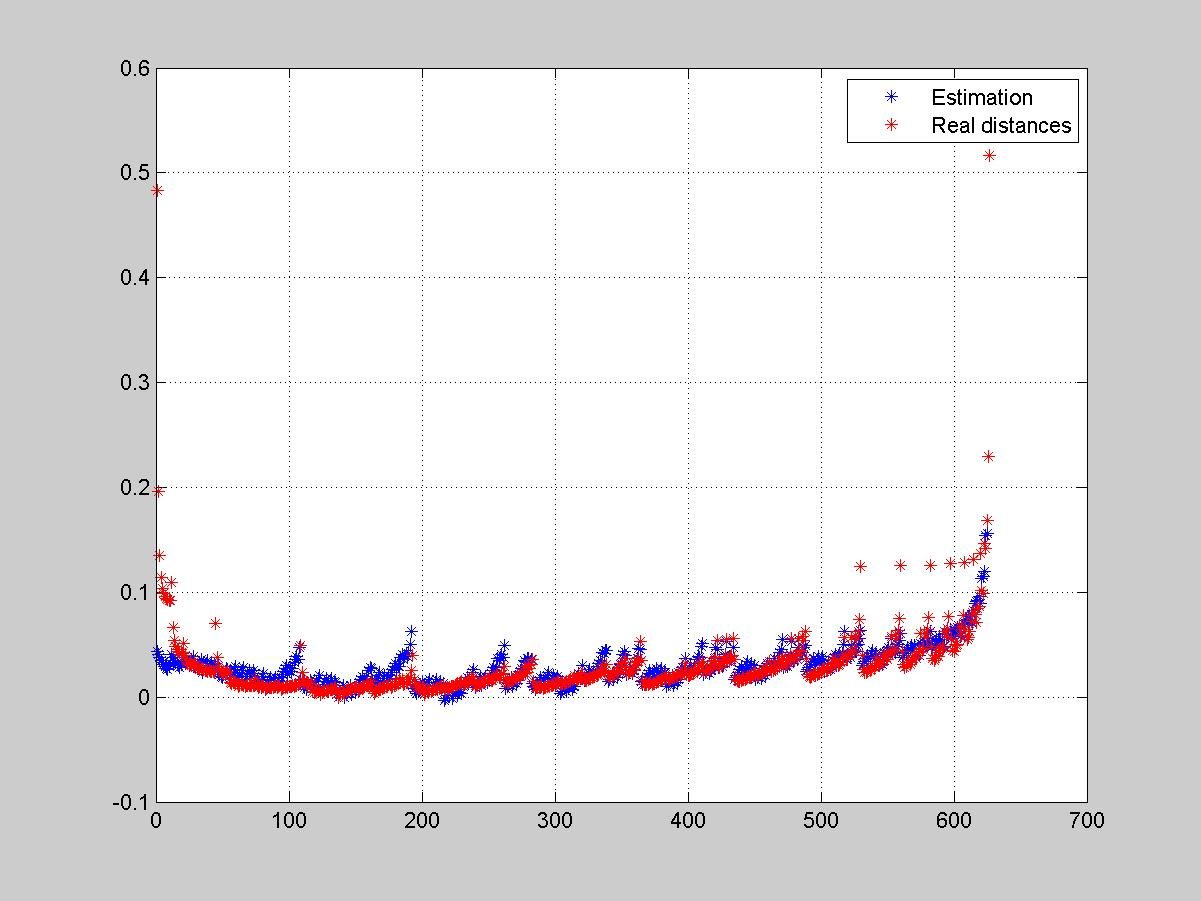
\includegraphics[scale=0.2]{MetricEstimation20Fabs}
\\Рис. 7. Расстояния от некоторой диаграммы до всех других диаграмм и их оценка по МНК. Слева оценка без модуля, справа взята оценка с модулем разниц строк: $dist(\lambda_1, \lambda_2) = \sum\limits_{i = 1}^n |c_i\Delta_i|$
\end{center}
\end{figure}

Посмотрим на вектор коэффициентов для обеих оценок (с модулем и без):
\begin{center}
\begin{tabular}{|c|c|c|c|c|c|c|c|c|c|c|}
\hline
Без модуля &-0.296 & -0.291 & -0.289 &-0.289 &... & -0.308& -0.317& -0.332 &-0.368 &-0.583\\
\hline
C модулем & 0.008 & -0.0004 & 0.0005 & 0.0013&...& 0.014 & 0.022& 0.035& 0.070 & 0.279  \\
\hline
\end{tabular}
\end{center}

Интересно, что в то время, как первые не меняют знак, вторые его чередуют (в номерах, попавших в многоточие имеется несколько отрицательных кэффициентов). 

На рисунке 8 представлена зависимость коэффициентов $c(i)$ для случая оценки с модулем и без. Похожа на экспоненциальную.
\begin{figure}[!ht]
\begin{center}
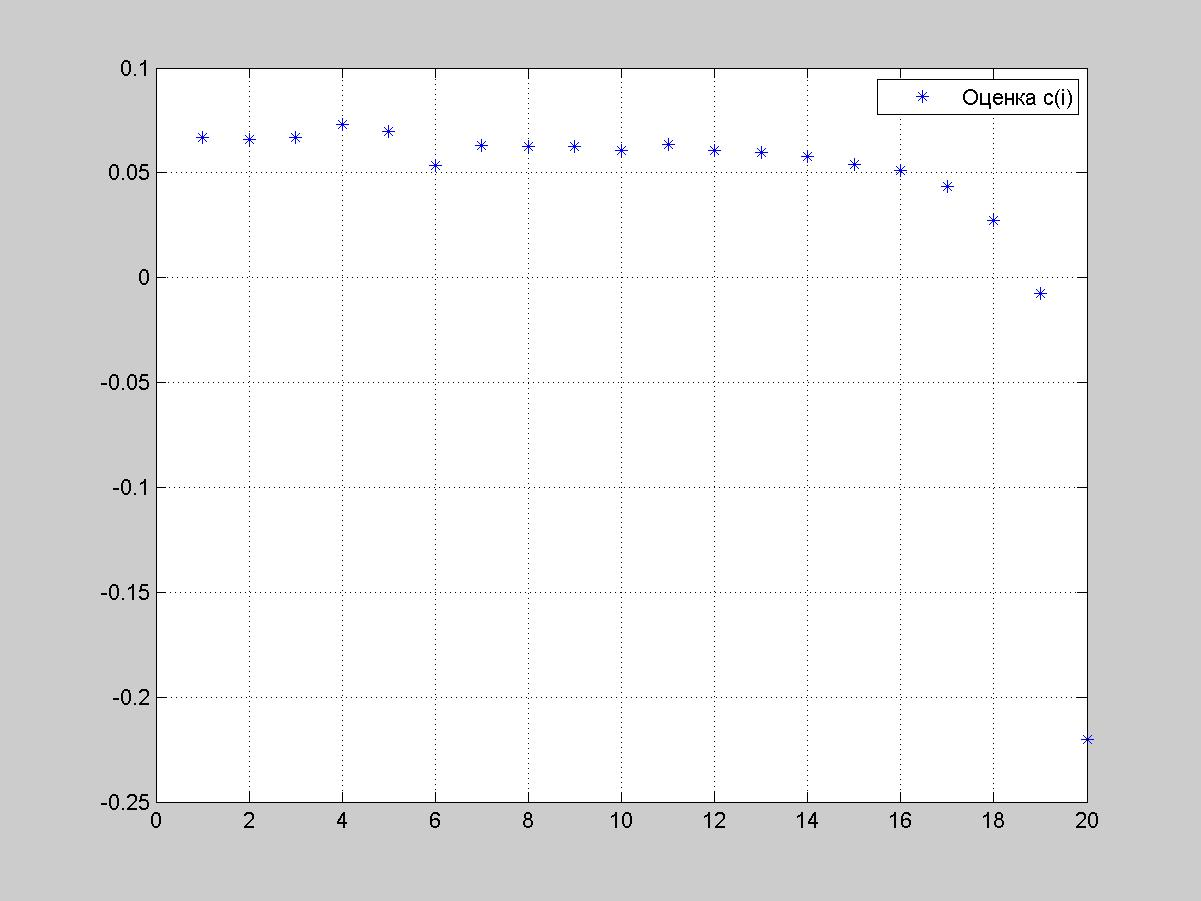
\includegraphics[scale=0.2]{CoefficientsEstimation20}
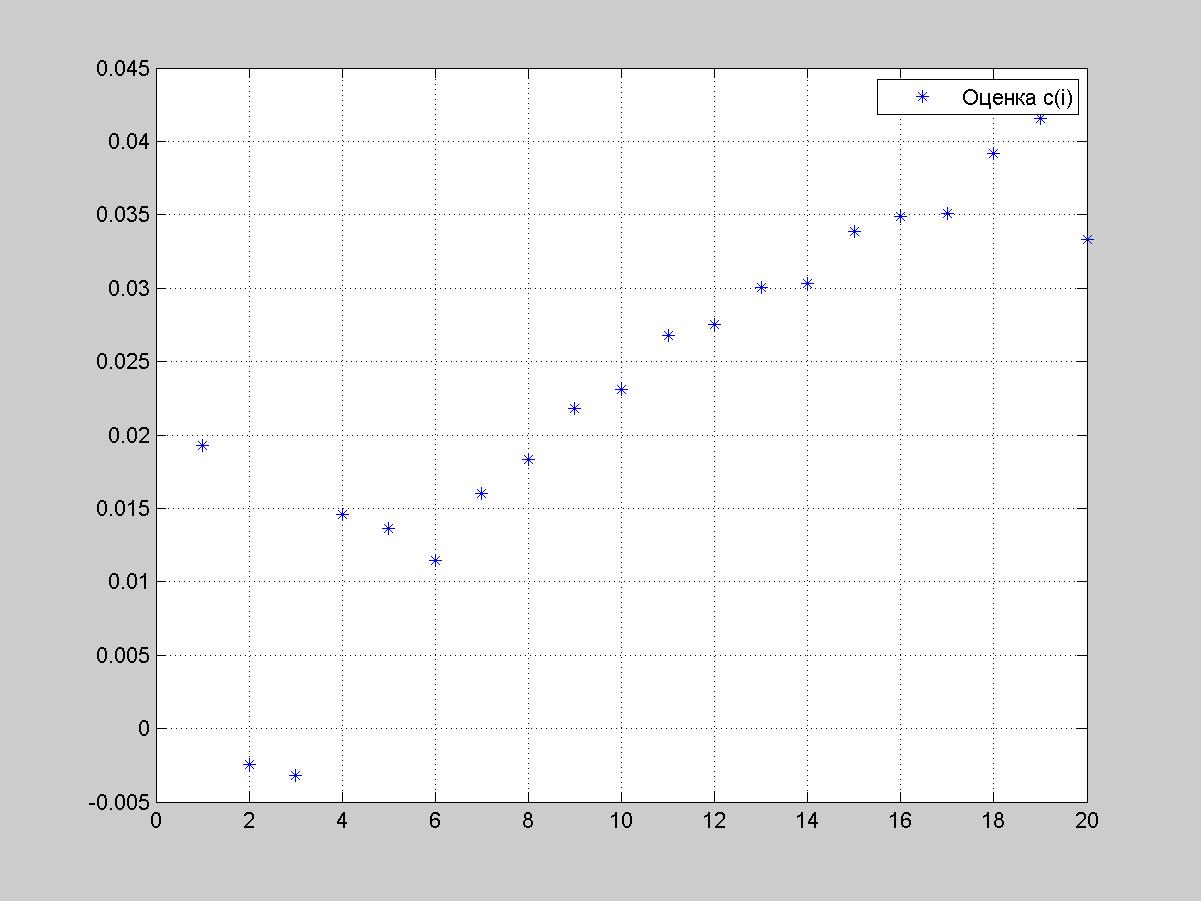
\includegraphics[scale=0.2]{CoefficientsEstimation20Fabs}
\\Рис. 8. Коэффициенты $c(i)$. Слева случай без модуля, справа случай оценки с модулем.
\end{center}
\end{figure}

\newpage
\subsection*{Нумерация трёхмерных диаграмм}
\hspace{\parindent}Для нумерации трёхмерных диаграмм можно было бы воспользоваться, например, формулой Макмагона. Однако, в данной работе я реализовал несколько другой способ нумерации, который описан ниже.
Идея следующая: рассмотрим  основание трёхмерной диаграммы Юнга и занумеруем его клетки простыми числами диагональным методом (см. рис. 9).

\begin{figure}[!ht]
\begin{center}
\includegraphics[scale=0.4]{Count3D}
\\Рис. 9. нумерация основания трёхмерной диаграммы.
\end{center}
\end{figure}

Рассмотрим теперь произвольную трёхмерную диаграмму $\lambda$ и покажем, как найти её номер. Обозначим через $p(x, y) : \mathbb{Z}^+ \times \mathbb{Z}^+ \rightarrow \mathbb{P}$  описанное выше отображение простых чисел в решетку. Пусть $h(x,y)$ - высота столбца $\lambda$, стоящего на клетке $(x,y)$. Для тех клеток $(x,y)$, на которых не стоят столбцы диаграммы, будем (как обычно и принято) считать $h(x,y) = 0$.
Тогда номер диаграммы $\lambda$ вычисляется по следующей формуле:
$$\No\lambda = \prod\limits_{(x,y) \in \mathbb{Z}^+ \times \mathbb{Z}^+}
 p(x,y)^{h(x,y) - max(h(x+1,y), h(x,y+1))} - 1$$

В силу того, что существует лишь конченое число клеток $(x,y) : h(x,y) \neq 0$, то данная формула позволяет эффективно вычислять номер диаграммы за конечное число шагов.

Нетрудно понять, что описанный способ нумерации задаёт биекцию между множеством диаграмм и множеством натуральных чисел. Действительно, рассмотрим произвольное число $n \in \mathbb{N}$ и укажем соответствующую ему диаграмму. Разложим $n$ на простые множители (это конечно не простая задача, но если рассматривать диаграммы с ограниченным числом клеток, то в общем решаемая за полиномиальное от числа максимальных клеток время). Далее, решаем треугольную систему линейных уравнений относительно высот столбцов, используя предыдущую формулу.

Данный алгоритм требует предподсчёта простых чисел до необходимого их количества (определяется тем, каково максимальное число клеток в нумеруемой диаграмме предполагается иметь). Если мы хотим нумеровать диаграммы из $n \leq N$ клеток, то необходимо предподсчитать первые $\frac{N(N+1)}{2}$ простых чисел и занумеровать ими клетки основания.

К минусам данной нумерации стоит отнести то, что она существенно немонотонна: сравнительное маленькие простые номера соответствуют огромным диаграммам (параллелепипедам с крайним столбцом, стоящим в соответствующей данному простому числу клетке). Поэтому, генерируя случайные числа для генерации случайных диаграмм, возможна частая генерация слишком больших диаграмм, которые не могут быть восстановлены по номеру. Кроме того, диаграммы, имеющие близкие номера, могут быть существенно различными и иметь существенно различное число клеток.

К плюсам данной нумерации можно отнести высокую скорость получения номера по диаграмме и диаграммы по номеру.

\newpage
\subsection*{Псевдоплашерелевский процесс в 3D}
\hspace{\parindent}С использованием для переходных вероятностей, аналогичную формуле в двухмерном случае для планшерелевского процесса (получающуюся из формулы крюков), реализовано случайное блуждание на трёхмерном графе Юнга.
На данный момент я использую то, что при добавлении очередной клетки к диаграмме почти никакие её крюки не меняются, и поэтому храню подсчитанный крюки для всех клеток, обновляя при добавлении клетки каждый раз только затронутые крюки, прибавляя к ним 1. Данный алгоритм требует по грубым оценкам $O(n^2\log(n))$ времени, где $n$ - размер конечной диаграммы.

Для получения более точной асимптотики я провёл серию экспериментов, последовательно генерируя диаграммы размером от 100 до 50000 клеток и замеряя время генерации. Ниже представлен график зависимости времени генерации от числа клеток диаграммы.

\begin{figure}[!ht]
\begin{center}
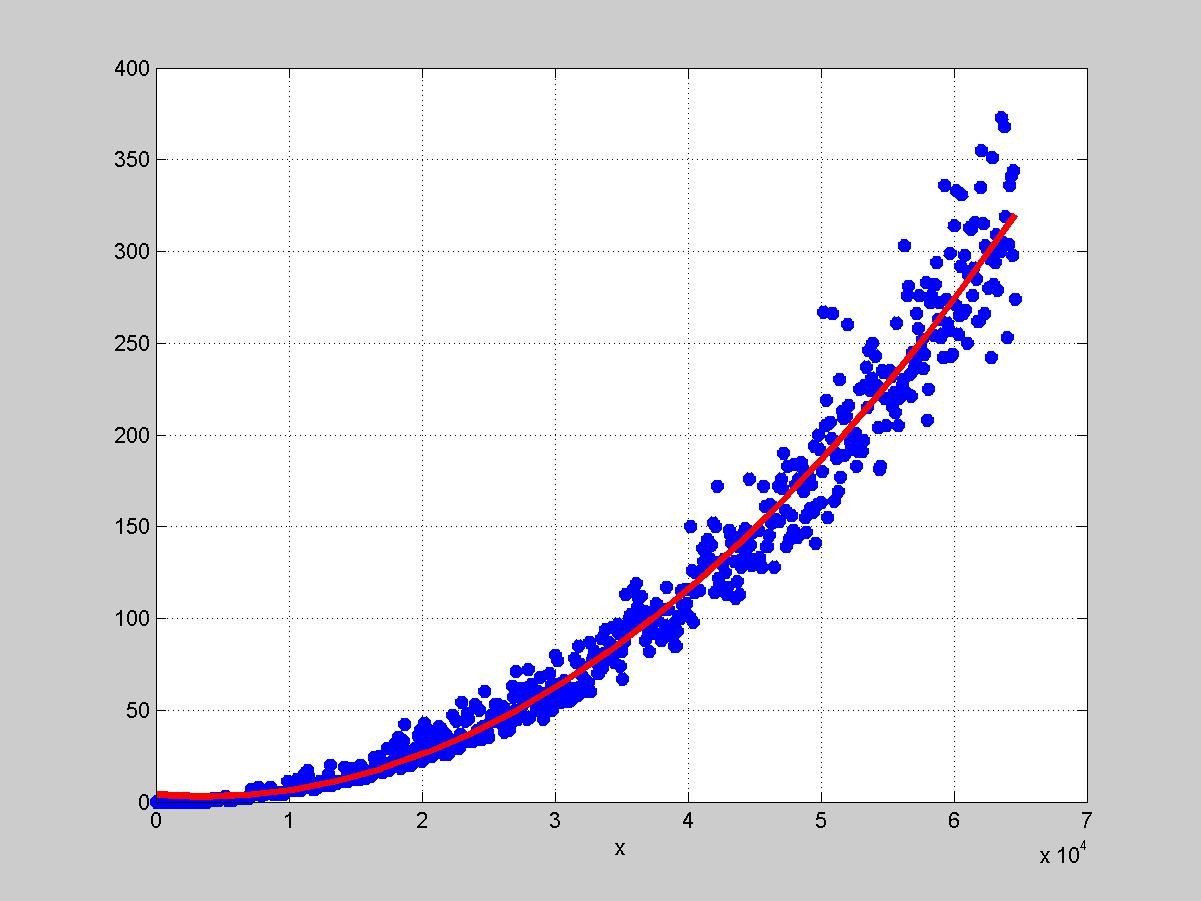
\includegraphics[scale=0.4]{AssymptHooksTime}
\\Рис. 10. Зависимость времени генерации случайной диаграммы по псевопланшерелевскому методу от числа клеток в итоговой диаграмме.
\end{center}
\end{figure}

Красная линия тренда является квадратичной функцией и приближает экспериментальную зависимость. По крайней мере, очевидно, что для миллиона клеток время будет порядка 1 дня расчётов, то есть при большом желании, достижимо.

За время порядка 15 минут удалось получить диаграмму из 100000 клеток, представленную на рисунке 11. Важной задачей сейчас будет приближённо задать её поверхность некоторой функцией от $(x,y)$.

\begin{figure}[!ht]
\begin{center}
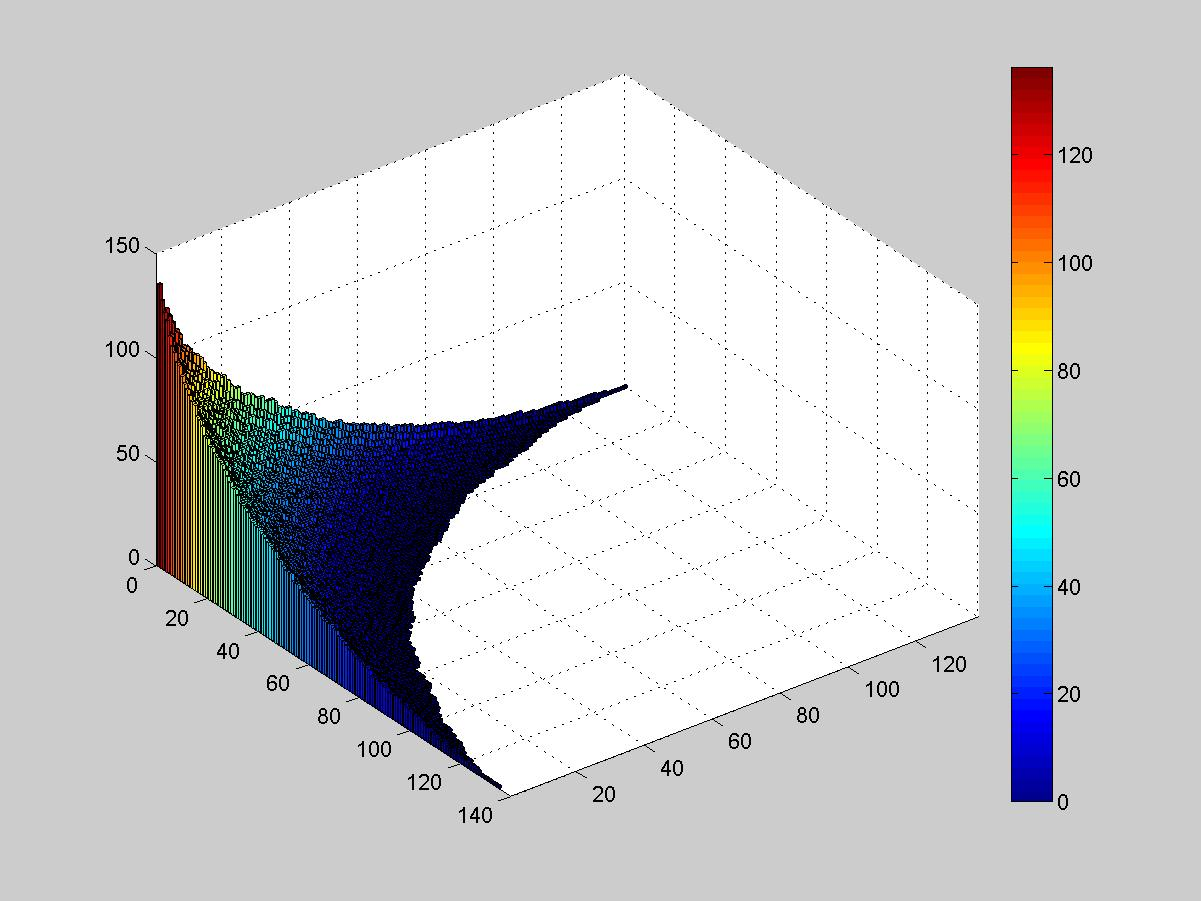
\includegraphics[scale=0.4]{3DHooks100000}
\\Рис. 11. нумерация основания трёхмерной диаграммы.
\end{center}
\end{figure}


\newpage
\section* {Нерешённые задачи}

\subsection*{Предельная форма трёхмерных диаграмм}
\hspace{\parindent} Николай Николаевич говорит, что было бы неплохо посмотреть, что будет, если использовать трёхмерный аналог формулы крюков для определения вероятностей перехода в трёхмерном случае (это уже будет не Планшерелевский процесс, ибо эта формула крюков в трёхмерном случае не даёт равновероятное появление любого пути до диаграммы). Попробовать возводить эти веса для переходных вероятностей в некоторые степени и посмотреть, будет ли меняться предельная форма. Посмотреть, что за кривые высекаются предельной диаграммой на координатных плоскостях. Видим, что зависимость скорее противоположная ожидаемой: коэффициенты растут с ростом индекса строки диагарммы Юнга.

\subsection*{Предельная форма двухмерных диаграмм}

\hspace{\parindent} Посмотреть, что будет, если возводить веса, найденные для Планшерелевских переходных вероятностей в малую отрицательную степень. При нулевой степени мы получаем процесс Ричардсона (очевидно, все веса 1), при положительных, больших 1, вроде как получаем того же Планшереля (Планшерель соответствует 1). При степенях от 0 до 1, я не помню, чему это соответствует, скорее всего тоже Планшерелю (надо проверить!).

\subsection*{Предложение Николая Николаевича}

Построение остовного дерева графа Юнга и Паскаля с использованием метрики Канторовича (видимо, предлагается использовать расширение метрики на весь граф, то есть научиться считать расстояния между вершинами с различных этажей графа).

\end{document}